\chapter{\IfLanguageName{dutch}{Stand van zaken}{State of the art}}
\label{ch:stand-van-zaken}

% Tip: Begin elk hoofdstuk met een paragraaf inleiding die beschrijft hoe
% dit hoofdstuk past binnen het geheel van de bachelorproef. Geef in het
% bijzonder aan wat de link is met het vorige en volgende hoofdstuk.

In dit hoofdstuk wordt de stand van zaken besproken.
Dit bevat wat er al onderzocht is rondom het gene wat er in deze bachelorproef besproken wordt.
De stand van zaken zorgt er voor dat een lezer die niet op de hoogte is van het besproken onderwerp kan volgen met na het lezen hiervan.

% Pas na deze inleidende paragraaf komt de eerste sectiehoofding.

%Dit hoofdstuk bevat je literatuurstudie. De inhoud gaat verder op de inleiding, maar zal het onderwerp van de bachelorproef *diepgaand* uitspitten. De bedoeling is dat de lezer na lezing van dit hoofdstuk helemaal op de hoogte is van de huidige stand van zaken (state-of-the-art) in het onderzoeksdomein. Iemand die niet vertrouwd is met het onderwerp, weet nu voldoende om de rest van het verhaal te kunnen volgen, zonder dat die er nog andere informatie moet over opzoeken \autocite{Pollefliet2011}.

%Je verwijst bij elke bewering die je doet, vakterm die je introduceert, enz. naar je bronnen. In \LaTeX{} kan dat met het commando \texttt{$\backslash${textcite\{\}}} of \texttt{$\backslash${autocite\{\}}}. Als argument van het commando geef je de ``sleutel'' van een ``record'' in een bibliografische databank in het Bib\LaTeX{}-formaat (een tekstbestand). Als je expliciet naar de auteur verwijst in de zin, gebruik je \texttt{$\backslash${}textcite\{\}}.
%Soms wil je de auteur niet expliciet vernoemen, dan gebruik je \texttt{$\backslash${}autocite\{\}}. In de volgende paragraaf een voorbeeld van elk.

%\textcite{Knuth1998} schreef een van de standaardwerken over sorteer- en zoekalgoritmen. Experten zijn het erover eens dat cloud computing een interessante opportuniteit vormen, zowel voor gebruikers als voor dienstverleners op vlak van informatietechnologie~\autocite{Creeger2009}.

\section{Schriftsystemen en hun groepen}

Onderzoek naar verschillende soorten schriftsystemen is simpel terug te vinden aangezien het beschouwd wordt als een echte wetenschap sinds de 20e eeuw.
Alhoewel het onderzoek vooral aanwezig was in de westerse wereld was er een soort van discriminatie aanwezig in dit vak.

Een van de eerste boeken over de verschillen in schriftsystemen was het boek genaamd 'A Study of Writing', geschreven door I. J. Gelb in 1952. \autocite{Gelb1952}
De schrijver trachtte een basis neer te leggen voor de ontwikkeling van een nieuwe wetenschap dat de naam 'grammatologie' zou gekregen hebben.
Deze nieuwe wetenschap probeerde standaard principes vast te leggen over het gebruik en de evolutie van het schrift op een vergelijkende wijze.
Dit was anders dan de voorgaande studies in het vak van schriftsystemen aangezien het een aantal systemen vergeleek met andere en niet enkel keek naar een systeem zijn geschiedenis en evolutie.
Dit boek bracht duidelijkheid in andere schriftsystemen dan dat de westerse bewoner gewoon was. 
In dit boek legde de schrijver uit hoe taalkundigen de gesproken taal zagen als iets dat meer biologisch is ontwikkeld en dit al doorheen de hele evolutie van de mens.
Daarentegen vermelde hij dat schriftsystemen zijn ontwikkeld als een technologie en dit enkel in de voorbije duizenden jaren en duidelijk meer een culturele dan een biologische schenking is.

In de jaren 60 waren er nog grote misopvattingen aanwezig bij de taalkundigen.
Bijvoorbeeld beschouwde Jack Goody, een toenmalig taalkundige,  het Chinese schrift als een gelimiteerd systeem aangezien hij vond dat het incapabel was om vele ideeën uit te drukken en hinderde de adoptie van westerse talen in deze cultuur.

Gelukkig is in de laatste jaren alles veranderd, de studie naar schriftsystemen is een gerespecteerde wetenschap in de taalkunde en is daarbij ook een beoefende wetenschap. 
Met dank aan de globalisatie is er een groter begrip gevormd voor andere talen dan die in de westerse wereld.
Aangezien het duidelijk is dat schriftsystemen ontwikkeld zijn uit de cultuur en niet uit de biologische geschiedenis is het interessanter om dit te bestuderen aangezien het nieuwer en flexibeler is.

Een schriftsysteem, technisch beschreven als een schrift of orthografie kan geclassificeerd worden onder verschillende groepen.  \autocite{David} \autocite{Allan2015}
Er zijn een aantal soorten groepen en allen zijn simpel van elkaar te onderscheiden maar in dit onderzoek wordt er gefocust op de 3 meest voorkomende.

Eén daarvan is het logografische schrift of anders verwoord, het beeldschrift.
Bij deze groep zijn volledige woorden uitgeschreven als een volledig teken dat compleet op zijn eigen staat en geen hulp nodig heeft van andere tekens om het te kunnen lezen.
Zoals hierboven reeds vermeld werd dit vroeger als een gelimiteerd schrift beschouwd aangezien het niet mogelijk is om een andere talen uit te drukken in dit schrift.
Dit is niet correct aangezien alle logografische schriften nooit puur logografisch zijn. Bij deze schriften is er naast woord-gebaseerde tekens ook klank-gebaseerde tekens voor het representeren van woorden die niet eigen zijn aan de taal of het schrift.
Het logografisch schrift wordt bekeken als een van de oudste groepen, de talen die onder deze groepen vallen zijn vaak ook oude schriften waardoor ze tijd hadden om zich volledig te ontwikkelen en zijn daardoor interessant in het heden.

Een andere groep is het syllabisch of lettergrepenschrift.
Bij deze schriften stellen de symbolen een klinker of een combinatie van medeklinkers en klinkers voor, simpeler gezegd stelt elk symbool simpelweg een lettergreep voor.
Lettergrepenschriften zijn vaak schriften die vroeger vooral werden gebruikt, in deze tijd komen deze schriften zelden voor.
een lettergrepenschrift komt deze tijd meer voor bij een logografisch schrift, dit zijn de klank-gebaseerde tekens zoals hierboven vermeld.

Onder deze groep valt er een andere groep die nog vaak voorkomt en niet mag weggelaten worden.
Deze groep is gekend als een consonantenschrift, deze schriften bestaan enkel uit medeklinkers waarbij de klinkers compleet worden genegeerd, hierdoor komt er bij het uitspreken van deze schriften wat gokken bij te pas en ervaring om de juiste klank te vinden.


De laatste en grootste is een groep dat vooral voorkomt in de westerse wereld en momenteel ook de meest gebruikte, het alfabetisch schrift.
De reden waarom dit de meest voorkomende groep is is omdat het een van de simpelste groepen is in vergelijking met de andere.
Het alfabetisch schrift representeert de fonologische structuur van de gesproken taal die dit schrift gebruikt, de geschreven taal representeert de uitgesproken klank.

Hier zijn er verschillen in de klank tussen de talen die dit schrift gebruiken, De Engelse uitspraak voor het woord 'hand' is bijvoorbeeld verschillend tegenover de Nederlandse uitspraak van dit zelfde woord.
Deze verschillen komen voort uit het uitspreken van dit schrift, vaak zijn ze te vinden in hoe de lippen, tong, gehemelte en keel wordt gebruikt. Bij alle uitgesproken talen worden deze verschillend gebruikt en vormen daardoor steeds een andere soort klank. 

Het alfabetisch schrift is er een die de andere schriften overtreft aangezien het fonologisch is, hiermee kunnen een groot deel van de reeds bestaande klanken worden uitgedrukt.
Een voorbeeld hiervan is het universele fonologische schrift dat bestaat uit een aantal symbolen die weergeven hoe een bepaald woord moet worden uitgesproken.
De klanken worden dan letterlijk uitgeschreven op papier en dit enkel op basis van gehoor.


\autocite{Rickandie2016} Het schrift is in de eerste vorm uitgevonden door Semitische volkeren met als bekendste de Feniciërs. Het alfabetisch schrift werd door veelvuldige contacten met omringende volken overgenomen door de Grieken, Hebreeërs en Arabieren. Via de Grieken namen ook de Romeinen het over. Gaandeweg hebben er echter veel aanpassingen plaatsgevonden tot het uiteindelijke eenvoudige schrift. De naam van het schrift is afgeleid van het Griekse alpha en bèta dat de eerste twee symbolen zijn van het Griekse alfabet.


\section{Artificiële intelligentie}

Aangezien het programma dat zal worden geschreven een aantal beslissing moet maken en kunnen nadenken over deze beslissing wijst dit automatisch op een technologische term, namelijk artificiële intelligentie.
Het mogelijk maken voor programma's om te denken, doen en leren als een mens.
Of een meer genuanceerde definitie.

Artificiële of kunstmatige intelligentie is een interdisciplinair concept dat de mogelijkheid bestudeerd voor het ontwikkelen van machines capabel om interactie aan te gaan met hun omgeving en in te werken op de ontvangen data op een manier die als intelligent beschouwd kan worden.

De term artificiële intelligentie werd als eerst gebruikt door John McCarthy in 1956, een Stanford onderzoeker.
Hij bedacht de term en legde AI vast als een branche van de computerwetenschap.

Artificiële intelligentie is in onze tijd al redelijk ontwikkeld en blijft maar groeien, het is tegenwoordig overal te vinden in het leven van de doodgewone mens.
Een eenvoudig voorbeeld hiervan is Siri of Alexa, een persoonlijke assistent. Deze en anderen zijn al in staat om onze stem te herkennen, de toegankelijke informatie te analyseren en een zo compleet mogelijk antwoord terug te geven. Deze assistenten leren voortdurend meer over hun gebruiker waardoor ze beter en gemakkelijker kunnen voldoen aan de persoonlijke eisen van de gebruiker.

Experten voorspellen dat artificiële intelligentie binnen het volgende decennia de mens zal overtreffen in het vervolledigen van simpele opdrachten zoals het vertalen van buitenlandse talen, het schrijven van verslagen of het besturen van een wagen. Maar het kunnen schrijven van een hooggewaardeerd boek of de taken overnemen van een chirurg zou nog iets wat langer kunnen duren. \autocite{Katja2018}
Voor deze twee is er verwacht dat deze vaardigheden mogelijk zullen zijn in respectievelijk 2049 en 2053.


\section{Machine Learning en Deep Learning}

Terwijl artificiële intelligentie, Machine Learning en Deep Learning vaak door elkaar worden gebruikt zijn er een aantal verschillen dat deze drie termen van elkaar onderscheid. Een manier om de relatie tussen deze te visualiseren is door middel van concentrische cirkels.
artificiële intelligentie is hierbij de overkoepelende cirkel en dan ook de buitenste laag die het gehele domein van de studie voorstelt, Machine Learning is dan een cirkel binnen in artificiële intelligentie. Als laatste heb je Deep Learning, de kleinste cirkel, dat een verfijning is van Machine Learning en representeert de meeste artificiële intelligentie applicaties die vandaag worden gebruikt.

Machine Learning is simpel uitgelegd het proces van het ontwikkelen van machines die in staat zijn datasets op te halen, algoritmes uit te voeren op deze data en vervolgens zichzelf te trainen en uiteindelijk waardevolle inzichten te ontwikkelen gebaseerd op deze datasets.
Het grootste verschil tussen Machine Learning en artificiële intelligentie is dat Machine Learning niet expliciet afhangt van de geschreven code van zijn ontwikkelaar. Machine Learning gebruikt eerder geschreven code als een startpunt en halen daarna data en informatie op waarop ze kunnen studeren, veel gelijkend op hoe een student zou studeren voor een examen.

\autocite{Arthur Samuel, 1959} "The ability to learn without being explicitly programmed."

De termMachine Learning werd voor het eerst gebruikt in 195 door Arthur Samuel,  was in de jaren 80 daarentegen kreeg het vak meer aandacht en werd er meer onderzoek in gestoken waardoor er een grote groei plaatsvond die nog altijd even sterk is in het heden. \autocite{KeithD.2019} 
Momenteel wordt Machine Learning vooral gebruikt bij het herkennen van gezichten, stemcommando's en het vertalen van talen. Vooral terug te vinden bij persoonlijke assistenten zoals Siri of Alexa, zoals hierboven vermeld.

Een voorbeeld van Machine Learning is het voorspellen van de prijs van een wagen.
De enigste taak dat Machine Learning moet volbrengen is het geven van een best passend antwoord maar met invloed van vele parameters, een model dat de prijs zou kunnen voorspellen van een wagen gaat als volgt.
Eerst en vooral kijkt het model naar een hoop data van andere wagens waar de prijs al van bekend is. 
In deze data komen vooral parameters terug die invloed hebben op de prijs van de auto zoals het merk, het jaar van productie, het aantal al afgelegde kilometers, de motor, de wielen, enzovoort. 
Uit deze parameters ontwerpt het model een voorspellingsfunctie, wanneer een prijs moet worden voorspelt van een wagen worden alle nodige parameters ingevoerd in deze functie en hieruit wordt een best passende prijs aan gegeven.

Dit soort van Machine Learning staat bekend onder gesuperviseerd leren waarbij er data is gegeven, je heb daarnaast ook niet-gesuperviseerd leren waarbij er geen data is gegeven en het model correlaties legt tussen data.
Bij het voorbeeld van de wagens zou het dus kunnen vaststellen bij 3 verschillende wagens dat wagen 1 meer gelijkenissen heeft met wagen 2 dan met wagen 3.
Als laatste onder Machine Learning heb je ook Reinforcement Learning waarbij een model beloningen krijgt voor de acties die het onderneemt. Bij een incorrecte actie krijgt het een negatieve beloning en bij een correcte actie krijgt het een positieve beloning, hieruit kan het model leren wat het wel en niet zou moeten doen.

Deep Learning is geïnspireerd door de structuur van het menselijke brein, het menselijk brein bestaat uit een complex netwerk van miljarden neuronen die met elkaar communiceren door middel van synapsen.
Deze neuronen sturen voortdurend elektrische impulsen waardoor het nodige informatie kan doorsturen naar andere delen van het lichaam, zoals de spieren of het hart.
Dit is gelijkaardig bij Deep Learning aangezien het gebruik maakt van artificiële neurale netwerken. In zo een netwerk is elk neuron capabel om een antwoord te geven op simpele ja/nee-vragen. Door vele neuronen in zo een dergelijk neuraal netwerk te implementeren kan zo een netwerk deftige antwoorden terug geven zonder het aanpassen van de geschreven code.

Het simpelste en oudste voorbeeld van een neuraal netwerk is een perceptron, een netwerk dat lineair classificeert dat wordt gebruikt voor binaire voorspellingen. Dit betekent dat de data lineair onderscheidbaar moet zijn. (Figuur \ref{tab:lineair})\\
Een perceptron, eigenlijk een neuron, bestaat uit een enkele laag, een invoer laag, bijkomende gewichten, een somfunctie en een activatiefunctie.
De invoerlaag krijgt de invoer en vermenigvuldigt deze met de bijkomende gewichten, deze worden dan ingevoerd in de somfunctie die een uitvoer doorgeeft naar de activatiefunctie die vervolgens bepaald of de finale uitvoer 0 of 1 bevat. (Figuur \ref{tab:perceptron})\\
Trainen van een perceptron gebeurt door middel van het invoeren van veel data met de gekende output, naarmate wijzigt het perceptron de gewichten zodanig dat een zo best passende output kan worden gegenereerd.

Een voorbeeld waar Deep learning voor gebruikt wordt en waar er enkel een simpel neuraal netwerk voor moet worden uitgebouwd is het herkennen van getallen.
Aangezien alle getallen enkel uit 10 verschillende figuren bestaat (van 0 tot 10) is het niet ingewikkeld om een onderscheid aan te leren. \autocite{Dann2010}


\begin{figure}
	
	
	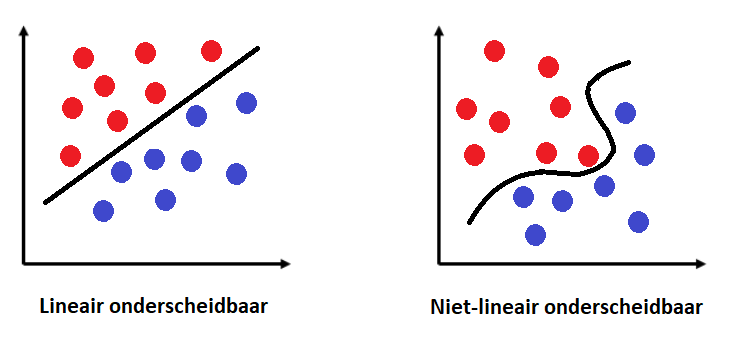
\includegraphics[width=\linewidth]{img/Lineair_onderscheidbaar.png}
	\caption{Lineair onderscheidbaar}
    \label{tab:lineair}
	
\end{figure}


\begin{figure}
	
	
	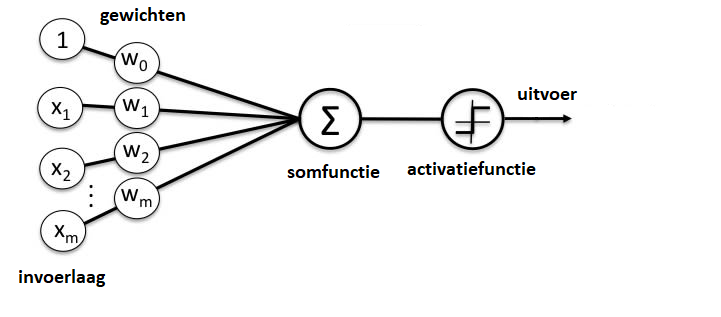
\includegraphics[width=\linewidth]{img/Perceptron.png}
	\caption{Architectuur van een Perceptron}
	\label{tab:perceptron}
\end{figure}

Een meer geavanceerd neuraal netwerk is een netwerk met meerdere lagen, waarbij elke laag een groot aantal aan neuronen bevat, de eerste laag is altijd de invoerlaag en de laatste laag is altijd de uitvoer laag, de gekende data wordt ingevoerd in de invoerlaag en vervolgens wordt er een resultaat berekend dat terug te vinden is in de uitvoerlaag. De daar in tussen liggende lagen worden 'hidden layers' genoemd, hierin krijgen de neuronen een invoer en produceren ze een gepaste uitvoer door middel van een activatie functie.
Elk neuron in een laag is vervolgens verbonden met elk neuron in de daaropvolgende laag waardoor de neuronen genoeg informatie krijgen om te beslissen welke output ze moeten doorgeven naar de volgende laag.

Neurale netwerken kunnen gebruikt worden bij fotoherkenning.
Neem nu een simpel voorbeeld van een artificieel neuraal netwerk dat moet beslissen of een foto een appel of een banaan bevat.
Het netwerk heeft drie verschillende vragen.


\begin{itemize}
	\item Is het voorwerp in de foto rond?
	\item Is het voorwerp in foto geel?
	\item Heeft het voorwerp in de foto een steel?
\end{itemize}

Bij een foto van een banaan zouden de neuronen antwoorden met respectievelijk neen, ja en neen. Voor een appel zou het antwoorden met respectievelijk ja, neen en ja. Met het gebruik van binaire getallen zou het netwerk aanleren dat de output voor een banaan 010 bevat en voor een appel 101.
Wanneer dit voorbeeld wordt uitgeschreven over een groot aantal neuronen lagen is het mogelijk om veel complexere problemen aan te pakken.

Deep Learning is een redelijk nieuwe term aangezien het pas voor het eerst werd gebruikt rond het jaar 2000. Sinds is het een veelgebruikte term en is het een regelmatig besproken onderwerp binnen het vak van artificiële intelligentie. \autocite{Goff2018}


\section{Convolutional Neural Network}

Een 'Convolutional Neural Network', ook bekend onder CNN of ConvNet, is een neuraal netwerk dat zich specialiseert in het verwerken van data dat roostervormig is, zoals een afbeelding. 


Een digitale afbeelding is een binaire representatie van visuele data. Het bevat een reeks van pixels geordend in een rooster waarbij de pixelwaarden aantonen hoe licht en de kleur die de pixel moet weergeven.

Een CNN bestaat, net zoals bij een normaal neuraal netwerk, uit een invoerlaag, een uitvoerlaag en een aantal tussenliggende lagen.
Maar wat een CNN een CNN maakt zijn de tussenliggende lagen waarvan sommige convolutioneel of pooling zijn, de twee belangrijkste lagen in een CNN.

\subsection{Convolutionele laag}




\begin{figure}
	
	
	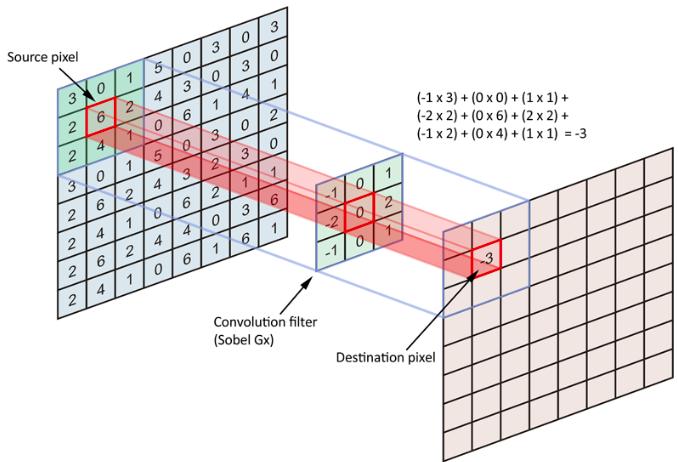
\includegraphics[width=\linewidth]{img/convolution.png}
	\caption{Het convolutional proces}
	\label{tab:convolutional}
\end{figure}

Het verschil tussen een convolutionele laag en een normale laag is dat convolutionele lagen 
lokale patronen in kleine roosters van twee dimensies, details dus, aanleert en een normale laag globale patronen aanleert over het geheel van de afbeelding.

Het grootste doel van een convolutionele laag is om randen, lijnen, vormen, enz. te herkennen.
Vanaf dat het zo een karakteristiek op een specifieke plaats heeft aangeleerd kan het het later in elke andere plaats herkennen. Terwijl een normale laag de karakteristiek opnieuw zou moeten aanleren.

Wanneer een tweede convolutionele laag volgt op een andere convolutionele laag kan de tweede laag aangeleerde patronen gebruiken van de voorgaande laag.
De tweede laag kan daardoor veel geavanceerde patronen aanleren, zoals een oog of een voetbal.

De convolutionele lagen werken met 3 dimensionale roosters, twee assen hiervan tonen de hoogte en breedte aan en de derde de diepte. Wanneer een afbeelding kleuren bevat zal deze diepte 3 bevatten, bij een zwart-wit foto zal deze 1 bevatten.

Een convolutionele laag is convolutioneel aangezien het een convolutionele operatie uitvoert.
Stel nu dat na een invoerlaag er een convolutionele laag is geplaatst
dan krijgt de convolutionele laag de niet verwerkte invoer binnen.
De laag maakt een of meerdere vensters aan, dat een filter wordt genoemd, met meegegeven hoogte en breedte, en per vak krijgt het een willekeurige waarde. Er kan veronderstelt worden dat deze filter verschuift over de gehele afbeelding. Voor elke positie dat de filter kan aannemen op de afbeelding is er een verbonden neuron.
Wanneer het venster enkele waarden in de afbeelding opneemt verwerkt hij dit met de willekeurige waarden en de uitvoer wordt in een nieuw rooster geplaatst  genaamd een 'feature map', de afbeelding wordt zodanig kleiner.(Figuur \ref{tab:convolutional})

Dit proces wordt duidelijker met een voorbeeld.
Gegeven is een afbeelding van grootte 32x32 (hoogte x breedte),
De afbeelding wordt ingevoerd in de convolutionele laag en deze maakt een filter aan met groote 3x3.
De aangemaakte filter krijgt zijn willekeurige waarden en begint links van boven bij de afbeelding, hier verwerkt de filter de waarden en plaatst ze in een nieuw rooster. 
Vervolgens schuift de filter met een stap naar rechts, wanneer deze filter niet meer naar rechts kan verschuiven, verschuift het met een stap naar beneden en begint opnieuw aan de linkerkant van de afbeelding.
Wanneer de filter op alle unieke posities is geweest is het nieuwe rooster gevormd. Bij dit voorbeeld heeft het nieuwe rooster een grootte van 30x30 aangezien dit het aantal unieke posities is dat de filter kan aannemen.
De convolutionele laag gebruikt voor elk neuron dezelfde filter, een filter kan een enkele karakteristiek herkennen, daarom wordt er aangeraden om meerdere filters te gebruiken in een convolutionele laag.
Wanneer meerdere filters worden gebruikt kunnen er meerdere karakteristieken worden herkent en zullen er betere resultaten worden opgeleverd.



\subsection{Pooling laag}

Naast de convolutionele lagen zijn ook de pooling lagen belangrijk in het proces van een CNN.
De pooling lagen worden meestal net na een convolutionele laag geplaatst, zo een laag versimpelt de informatie die verkregen werd door de convolutionele laag door een compactere versie te maken van deze informatie.
Er zijn twee manieren waarop een pooling laag dit kan doen, max-pooling en average-pooling, de meeste gebruikte hiervan is de eerste.

De pooling laag maakt zoals bij een convolutionele laag een filter van meegegeven grootte, vervolgens begint de filter in de hoek links van boven en neemt, bij max-pooling, de grootste waarde in de filter en plaatsts deze vervolgens in een nieuw rooster. Wanneer dit is voltooid schuift de filter door naar een volgende positie maar overlapt niet met informatie waar het al is geweest, in tegenstelling tot de filter bij een convolutionele laag.
Bij average-pooling neemt de filter het gemiddelde van de waardes die te zien zijn in de filter.
Stel nu dat de meegegeven hoogte en breedte 2 bevat, dan zal het verwerkte rooster half zo groot zijn als het originele rooster.(Figuur \ref{tab:pooling})\\
Zoals hierboven vermeld heeft een convolutionele laag vaak meerdere filters, wanneer we een pooling laag introduceren in het neuraal netwerk zal het evenveel pooling filters bevatten als convolutionele filters.

\begin{figure}
	
	
	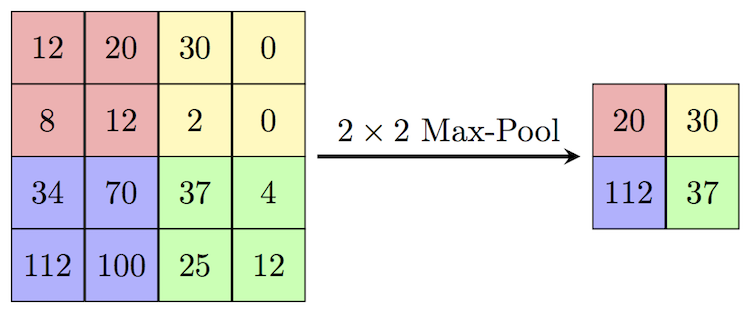
\includegraphics[width=\linewidth]{img/pooling.png}
	\caption{Het max-pooling proces}
	\label{tab:pooling}
\end{figure}

\section{Karakterherkenning}

Een convolutioneel neuraal netwerk kan voor een aantal onderwerpen gebruikt worden zoals, stemherkenning, classificatieproblemen \autocite{Yann1997}, het herkennen van handgeschreven zip code waarden\autocite{J.S.}, enzoverder.
Een onderwerp waarvoor convolutionele neurale netwerken veelal voor gebruikt wordt is karakterherkenning of OCR (Optical Character Recognition), een technologie waarbij uit een afbeelding of tekstdocument alle tekens uit het bestand kunnen worden herkend en apart kan worden opgeslagen.
Een voorbeeld hiervan is nummerplaatherkenning bij flitspalen. waarbij een foto wordt getrokken, en vervolgens wordt opgeslagen onder de herkende nummerplaat.
Karakterherkenning kan ook te pas komen bij het herkennen van handgeschreven karakters, een probleem dat hierbij voorkomt is dat schriften vaak kunnen variëren in stijl maar dezelfde patronen komen vaak terug.
Dit probleem kan dus opgelost worden met een convolutioneel neuraal netwerk aangezien dit deze vaak terugkomende patronen kan onthouden en simpelweg kan herkennen op andere plaatsen dan de originele gevonden plaats.

Wanneer onderzocht wordt naar karakterherkenning met behulp van een CNN zullen de onderzoekers vaak trachten karakters of woorden te herkennen uit een specifiek schriftsysteem. \autocite{Yoshua}\autocite{Yann}
Even zoeken op het internet en vele artikels kunnen teruggevonden worden die dit specifiek onderzoek toepassen, zoals het herkennen van woorden in het Latijnse schrift \autocite{Aiquan2012}, het herkennen van Chinese karakters \autocite{Weixin}, het herkennen van het Bengaals alfabet, een schriftsysteem uit Zuid-Azië \autocite{Mahbubar2015}, enzovoort.
Deze onderzoek trachten verschillende karakters uit een gekozen schriftsysteem te herkennen en zodanig woorden te vormen en uiteindelijk deze te lezen. Dit proces is simpelweg het lezen van tekst door middel van een CNN, wat vooral gebruikt kan worden bij het lezen van onbekende schriftsystemen maar veronderstelt dat het gebruikte schriftsysteem al gekend is.

Deze veel voorkomende onderzoeken zijn uitermate interessant aangezien het een beeld heeft van wat er mogelijk is en wat niet.
De onderzoeken volgen meestal dezelfde werkwijze, eerst en vooral wordt er voldoende data verzamelt van het specifieke schriftsysteem. Dit meestal uit al bestaande datasets.
Wanneer men spreekt over datasets zijn er twee groepen te onderscheiden, online datasets en offline datasets.
Bij een online handgeschreven karakter dataset zijn de opgeslagen karakters met wanneer de 'gebruikte pen' werd opgeheven en wanneer het werd neergezet, dit kan bijvoorbeeld komen door het gebruik van een smartphone waarbij de 'gebruikte pen' de vinger op het scherm is. \autocite{Cheng-Lin2011}
Een voorbeeld hiervan is de CoMNIST dataset, een dataset bestaande uit het Latijnse schriftsysteem en het Cyrillische. Bij deze dataset kan iedereen participeren met de opslag van de handgeschreven karakters.
De ontwerpers van de dataset maakten een website aan waarbij je een opgegeven letter krijgt, deze letter moet je vervolgens tekenen in een venster en deze wordt opgeslagen in de dataset.
Een offline dataset daarentegen bestaat uit data die gelezen is uit documenten of afbeeldingen, deze zijn vaker niet handgeschreven maar niet altijd.

Om verder te gaan op de veelgebruikte werkwijze in de al bestaande onderzoeken is de volgende stap het verwerken van de datasets zodanig dat het simpelweg gebruikt kan worden voor de volgende stap.
Hoe een dataset verwerkt wordt hangt af van de technologieën die worden gebruikt en persoonlijke preferentie.
In een bepaald onderzoek worden de afbeelding geroteerd, verschoven en uitgerekt om zodanig lokale vervorming te creëren, hierdoor komt er meer variëteit in de data. \autocite{Weixin}
Wat vooral voorkomt is het veranderen van de grootte van de data specifiek voor de verwachte invoer van het gebruikte model. \autocite{Aiquan2012} \autocite{Mahbubar2015}
Aan het einde van de nodige aanpassingen van de data volgt er vaak een laatste stap, namelijk de normalisatie van de te gebruiken data.
Normalisatie is het aanpassen van alle data zodanig dat de waarden van alle bijkomende variabelen op een zelfde schaal terecht komen.

De volgende stap is het aanmaken van het model, er wordt gezocht naar de lagen die de beste resultaten op zullen leveren en zorgen dat elke laag de correct invoer krijgt.
Wanneer het model is aangemaakt wordt het getraind met de verwerkte datasets, wanneer dit is gebeurd wordt het model getest en de resultaten worden neergeschreven.

Bij elk onderzoek is er zoals verwacht een conclusie uitgeschreven, in de meeste conclusies wordt er uitgelegd dat het gelukt is om een model te schrijven voor hun karakterherkenning.
Maar de inhoud van de conclusies bevatten vaak een redenering dat hun model nog kan worden verbeterd. \autocite{Ahmed2017}
Eén onderzoek blinkt hier wel in uit, dit onderzoek concludeert dat ze een hoge accuraatheid hebben bereikt met hun model. Het verschil met de andere onderzoeken is dat zij niet enkel een CNN gebruiken maar andere technologieën gebruiken, dit zijn vooral technologieën die gebruikt worden voor hun datasets. \autocite{Yann}

\section{Schriftherkenning}

Rond het kader van karakterherkenning valt er veel onderzoek terug te vinden, dit vooral in verband met karakterherkenning van specifieke schriftsystemen.
Een specifieker onderzoeksthema rond het kader van karakterherkenning is het kunnen onderscheiden van verschillende schriftsystemen, dit onderzoeksthema is weinig onderzocht maar kan een groot voordeel bieden aan het onderzoek van karakterherkenning.
Dit vooral wanneer er documenten moeten worden ontcijferd die meerdere schriftsystemen bevat. Een simpel voorbeeld hiervan is in de Japanse letterkunde, deze gebruiken verschillende schriftsystemen. Wanneer deze van elkaar onderscheiden kunnen worden in een document zou het vervolgens eenvoudiger worden om deze te vertalen met een ander karakterherkenningsysteem aangezien het gebruikte schriftsysteem al gekend zou zijn.

Wanneer er wordt gekeken naar het al onderzochte in verband met het herkennen van verschillende schriftsystemen is de gebruikte werkwijze gelijkaardig aan de werkwijze dat de onderzoeken gebruiken bij het identificeren van karakters bij een specifiek schriftsysteem.
De data wordt verzameld en verwerkt zodanig dat het kan ingevoerd worden in het aangemaakte model, dat de volgende stap inhoud.
Uiteindelijk wordt het model getest en is er een bijhorende conclusie aanwezig.

In de teruggevonden onderzoeken is de conclusie steeds positief, er is een hoge accuraatheid bereikt bij de testen maar er zijn nog enkele misvattingen van het model. Dit verklaren ze aangezien een aantal schriftsystemen dezelfde karakters delen. \autocite{Adman2015}

De gebruikte data bestaat uit afbeeldingen van volledige woorden \autocite{Baoguang2015} of van volledige paragrafen \autocite{Guo2009}.
Dit zorgt ervoor dat het model enkel gebruikt kan worden op volledige woorden of volledige paragrafen, wanneer een enkel karakter zal proberen herkend worden zal dit minder accurate resultaten opleveren.
Dit kan wel een oplossing bieden voor het probleem waarbij een aantal karakters worden gedeeld tussen verschillende schriftsystemen.
Wanneer het model wordt getraind op volledige woorden of paragrafen en zo een karakter tegenkomt, die ook voorkomt in andere schriftsystemen, kan het kijken naar de andere karakters die ook voorkomen in het woord of de paragraaf.

Bij een aantal schriften kan het voorvallen dat een groot aantal karakters ook gebruikt wordt door andere schriften.
Een voorbeeld hiervan is het Kanji, het schriftsysteem gebruikt in Japan, en het Hanzi, het schriftsysteem gebruikt in China.
Het Kanji heeft een groot aantal karakters van het Hanzi geadopteerd, vervolgens ondergingen beiden hun eigen evolutie en zijn er momenteel kleine verschillen tussen de twee schriften maar het is nog steeds ingewikkeld om ze van elkaar te onderscheiden. \autocite{Koichi2010}

Onder de terug gevonden artikels gebruikt enkel een hiervan een convolutioneel neuraal netwerk \textcite{Baoguang2015}.
Dit artikel concludeert dat het hoge resultaten behaalt met het gebruik van een CNN.

Onderzoek naar het kunnen herkennen van een alleenstaand karakter is niet teruggevonden, steeds trachten de artikels volledige woorden of paragrafen te herkennen.


















